\documentclass[../../main.tex]{subfiles}
\graphicspath{{images/Akustik/}{../../images/Akustik/}}
\begin{document}
\subsection{Akustik}
In diesem Kapitel wird auf die Implementierung der technischen Komponente 'Akustik' eingegangen. Die akustische Ausgabe einer Zahl eine Teilanforderung für den korrekten Ablauf von Pren. Während der Fahrt wird ein Signal mit einer Nummer gelesen, diese Nummer wird am Ende der Fahrt akustisch wiedergegeben.

\subsubsection{Anforderung}

\paragraph{Anforderungen}
\begin{itemize}
    \item Zahl akustisch wiedergeben (Speaker oder Buzzer)
    \item Korrekte Zahl wird wiedergegeben
    \item Kompakt
    \item Günstig
    \item Keine eigene Stromquelle
    \item Verständliche Ausgabe
\end{itemize}

\subsubsection{Lösung}
Die Lösung entspricht dem Lösungskonzept aus Pren1. Sobald ein Signal, in Form einer Zahl von 1-10, erhalten wird, buzzt der Buzzer die entsprechende Anzahl.

\paragraph{Technologien / Komponente}
Über die GPIO Header des Raspberry Pi kann der Buzzer direkt angesprochen und versorgt werden. Ein einzelnes Signalkabel reicht für die Kommunikation aus.

Softwaretechnisch wird das Ganze mit Python ausgeführt. Python besitzt mächtige Bibliotheken in diesen Bereichen.

\subparagraph{Buzzer}
Es gibt zwei Arten von Buzzer, den Aktiv-Buzzer und den Passiv-Buzzer. Wir verwenden einen Passiv-Buzzer, der exakte Unterschied der beiden Modelle ist mir nicht bekannt, jedoch ist dies für die Implementierung nicht relevant. Für den Passiv-Buzzer gibt es viele Beispiele auf dem Internet. 

Auf dem Zug befindet sich der Buzzer zwischen Kran und dem Abstellplatz für den Würfel. Grösse und Gewicht erlauben eine einfache Montur auf einem Klettstreifen.

\subparagraph{GPIO}
Anbindung des Buzzers an den Raspberry Pi 3 B+ via GPIO Bus.

\begin{figure}[H] \centering
    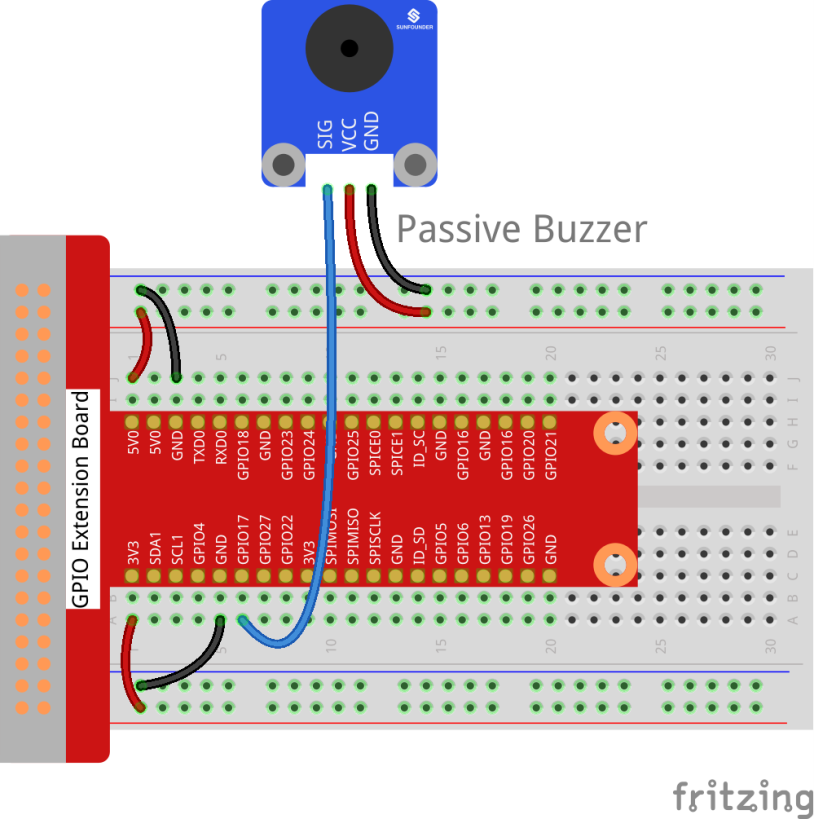
\includegraphics[width=0.5\textwidth]{VerkabelungAkustik}
    \caption{Verkabelung Buzzer}
    \label{fig:Buzzer}
\end{figure}
\begin{table}[H]
    \begin{center}
    \begin{tabular}{lll}
    \hline
    Bezeichnung     & GPIO Header & Buzzer \\ \hline
    Stromversorgung & 3V3      & VCC    \\ \hline
    Ground          & GND      & GND    \\ \hline
    Signal          & GPIO17   & SIG    \\ \hline
    \end{tabular}
    \end{center}
\end{table}

\paragraph{Prozessablauf}

\paragraph{Soll-Ist-Vergleich}
Der Buzzer wurde bereits in Pren1 getestet, dementsprechend ist das Ergebnis gemäss den Erwartungen.

\subsubsection{Entwicklungsablauf}
Logik und Aufbau für die Kommunikation mit dem Buzzer war bereits aus Pren1 vorhanden. Die Herausforderung lag lediglich in der Kommunikation mit der Applikation. Der Buzzer wurde mithilfe einer Akustik-Klasse an die Middleware gebunden. Zuletzt wird die WebApp mit einer Akustik-Schnittstelle erweitert, welche das Senden von Akustik-Signalen erlaubt. 

\subsubsection{Testing}
Über die Akustik-Schnittstelle auf der WebApp kann der Buzzer jederzeit getestet werden.

\subsubsection{Reflexion}
Es gab keine bösen Überraschungen und der Buzzer läuft zuverlässig. Mit der kompakten Struktur und dem geringen Stromverbrauch ist er eine ideale Komponente für Projekte dieser Grössenordnung.

\end{document}